\documentclass[svgnames]{standalone}

\usepackage{tikz,mathtools}

\def\V{10}\def\p{7}

\begin{document}
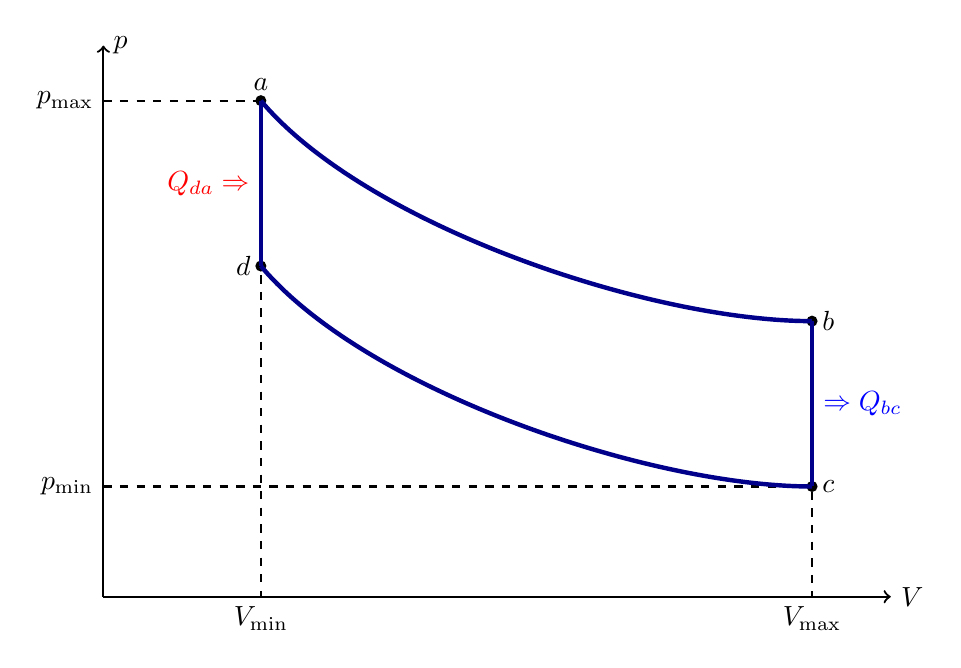
\begin{tikzpicture}[thick]
  \draw[->] (0,0) -- (0,\p) node[right] {$p$};
  \draw[->] (0,0) -- (\V,0) node[right] {$V$};

  \draw[dashed] (0,0.9*\p) node[left] {$p_\text{max}$} -| (0.2*\V,0) node[below] {$V_\text{min}$};

  \draw[dashed] (0,0.2*\p) node[left] {$p_\text{min}$} -| (0.9*\V,0) node[below] {$V_\text{max}$};

  \coordinate[label=above:$a$] (a) at (0.2*\V,0.9*\p);
  \coordinate[label=right:$b$] (b) at (0.9*\V,0.5*\p);
  \coordinate[label=right:$c$] (c) at (0.9*\V,0.2*\p);
  \coordinate[label=left:$d$] (d) at (0.2*\V,0.6*\p);

  \foreach \point in {a,b,c,d}
  \fill (\point) circle (2pt);

  \draw[ultra thick,DarkBlue] (a) edge[out=-50,in=180,looseness=0.7] (b) (b) -- (c) node[midway,right,blue] {$\Rightarrow Q_{bc}$} (c) edge[out=180,in=-50,looseness=0.7] (d) (d) -- (a) node[midway,left,red] {$Q_{da} \Rightarrow$};

\end{tikzpicture}
\end{document}